\section{Test Procedures}

\begin{figure}
	\centering
	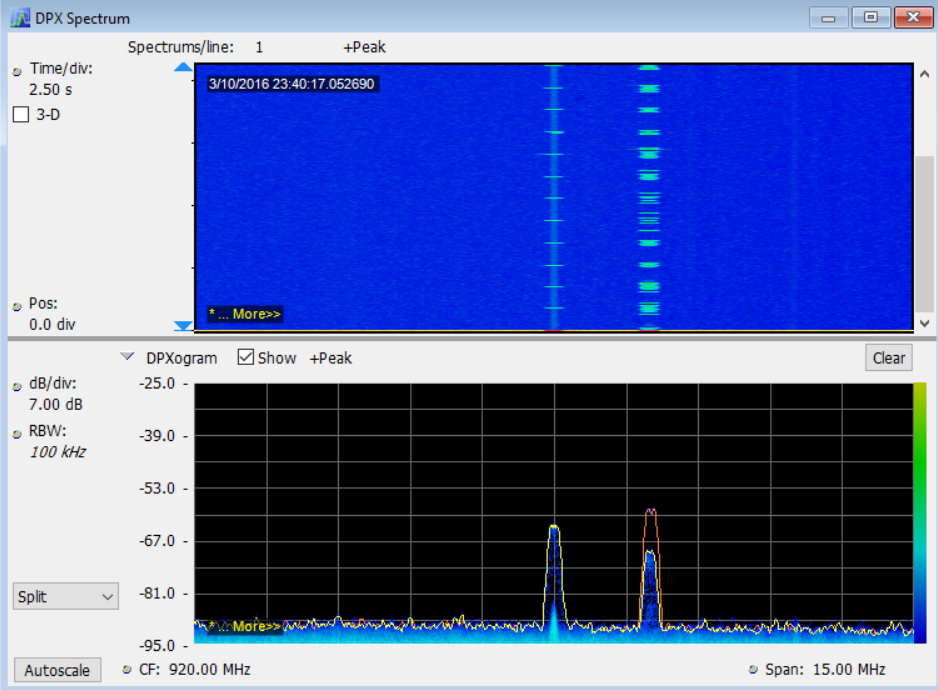
\includegraphics[scale=0.4]{FrequencyShift922-920}
	\caption{The result of using ALFRED to shift frequencies. One Node is left behind as the others move to the new channel.}
	\label{fig:freqshift}
\end{figure}


\begin{figure*}
	\centering
	\includegraphics[scale=0.5]{HopMessSmallest}
	\caption{The configuration used for the first set of tests.}
	\label{fig:HopMess}
\end{figure*}

\begin{figure*}
	\centering
	\includegraphics[scale=0.5]{NodeDrop}
	\caption{The configuration used for the second set of tests.}
	\label{fig:NodeDrop}
\end{figure*}

In order to characterize the platform we run three sets of tests presented below. The first test characterizes data hopping from one node to the next. The second test demonstrates batman-adv ability to switch routes based on the quality of each node. The final tests were used to examine A.L.F.R.E.D.'s ability to be used for exchanging frequency information from node to node. 

\subsection{Network Benchmarks}



For the first test we wanted to investigate the overhead each node adds to to the network. To test this, we arranged the USRPs in a line so that each node only had one route to the following nodes. This setup is shown in Figure \ref{fig:HopMess}. To ensure that nodes could only talk to their immediate neighbors, we staggered the transmit and recieve frequencies in order to force the network into the configure we wanted. We then tested the setup at three different sets of frequenies, all within the ISM Band. We used different sets of ping tests in order to determine the number of dropped packets and the time it took to send the packets. We used a total of 5 nodes. To get a baseline for the test, we setup two usrps and did not configure batman-adv on these nodes. This would help to get a clearer understanding of what the hardware limitations are of the USRPs. 


\subsection{Route Changes}

In a typical mesh environment, there will usually be more than one route from a source to a destination. In a traditional network, Batman-adv does a good job of switching routes based on the quality of links. This test was used to see if the same features would work in a cognitive environment. We initially setup four SDRs, a source, a destination, and two nodes that connect them. We give a much larger gain to the first node, in order to see if Batman-adv will recognize that this is a stronger path to the destination. Then, once the route is place into the routing table, we lower the gain to 0 and make it disappear. We then see if batman-adv is still able to find the new route even though it is running on a USRP. This setup is shown in Figure \ref{fig:NodeDrop}.



\subsection{Frequency Changes}

In the final test, we looked to see if A.L.F.R.E.D. would properly relay frequency information in order to keep the network communicating as the frequency increased and decreased. The user would increase or decrease the frequency using the web interface in order to simulate a cognitive radio making a decision to change to a new setting. If A.L.F.R.E.D. was able to exchange the information properly, then the network would still show all connected nodes, and the new frequency should be visible on the spectrum analyzer. If A.L.F.R.E.D. was not able to relay the information to all nodes, then we would lose nodes as some change to the new frequency while others remain. This would be reflected in the output from the spectrum Analyzer. 